%
% Sección de resultados de compraciones de desempeño.
% Artículo sobre tokenización.
%
% Proyecto Lovelace.
%

\section{Resultados y conclusiones}

En la tabla \ref{tabla:tiempos_tokenizacion} y la figura
\ref{figura:tiempos_tokenizacion} se muestran los resultados en tiempo de
las ejecuciones de los algoritmos presentados en secciones
anteriores\footnote{También se hizo la implementación de un DRBG como lo
describe el NIST en \cite{nist_aleatorios}}. Estos se llevaron a cabo en una
computadora con las siguientes características:

\begin{itemize}
  \item \textbf{Procesador:} Intel i5-7200U (2.5 GHz) de 4 núcleos.
  \item \textbf{Sistema operativo:} Arch Linux, kernel 4.17.
  \item \textbf{Base de datos:} MariaDB 10.1.
  \item \textbf{Compilador:} GCC 8.1.1
\end{itemize}

% Que los irreversibles sean más lentos resulta contraintuitivo: uno esperaría
% que como los reversibles deben de poder hacer la operación inversa por sí
% solos, entonces su operación sea más compleja. En realidad sospecho que así
% es, sin embargo la operaciones con la base de dato son muy lentas.
% Creo que antes de escribir la conclusión en serio, voy a tomar tiempos
% sin base de datos, solo de tokenización.

Claramente se puede notar que los métodos reversibles son más rápidos que los
irreversibles. 

\begin{table}
  \begin{center}
    \caption{Comparación de tiempos de tokenización.}
    \label{tabla:tiempos_tokenizacion}
    \begin{tabular}{|c|c|c|}
      \hline
      Algoritmo & Tokenización ($\mu$s) & Detokenización ($\mu$s) \\
      \hline
      FFX & 83 & 64 \\\hline 
BPS & 247 & 127 \\\hline 
TKR & 46260 & 373 \\\hline 
AHR & 3427 & 390 \\\hline 
DRBG & 54060 & 387 \\\hline 

    \end{tabular}
  \end{center}
\end{table}

\begin{figure}
  \begin{center}
    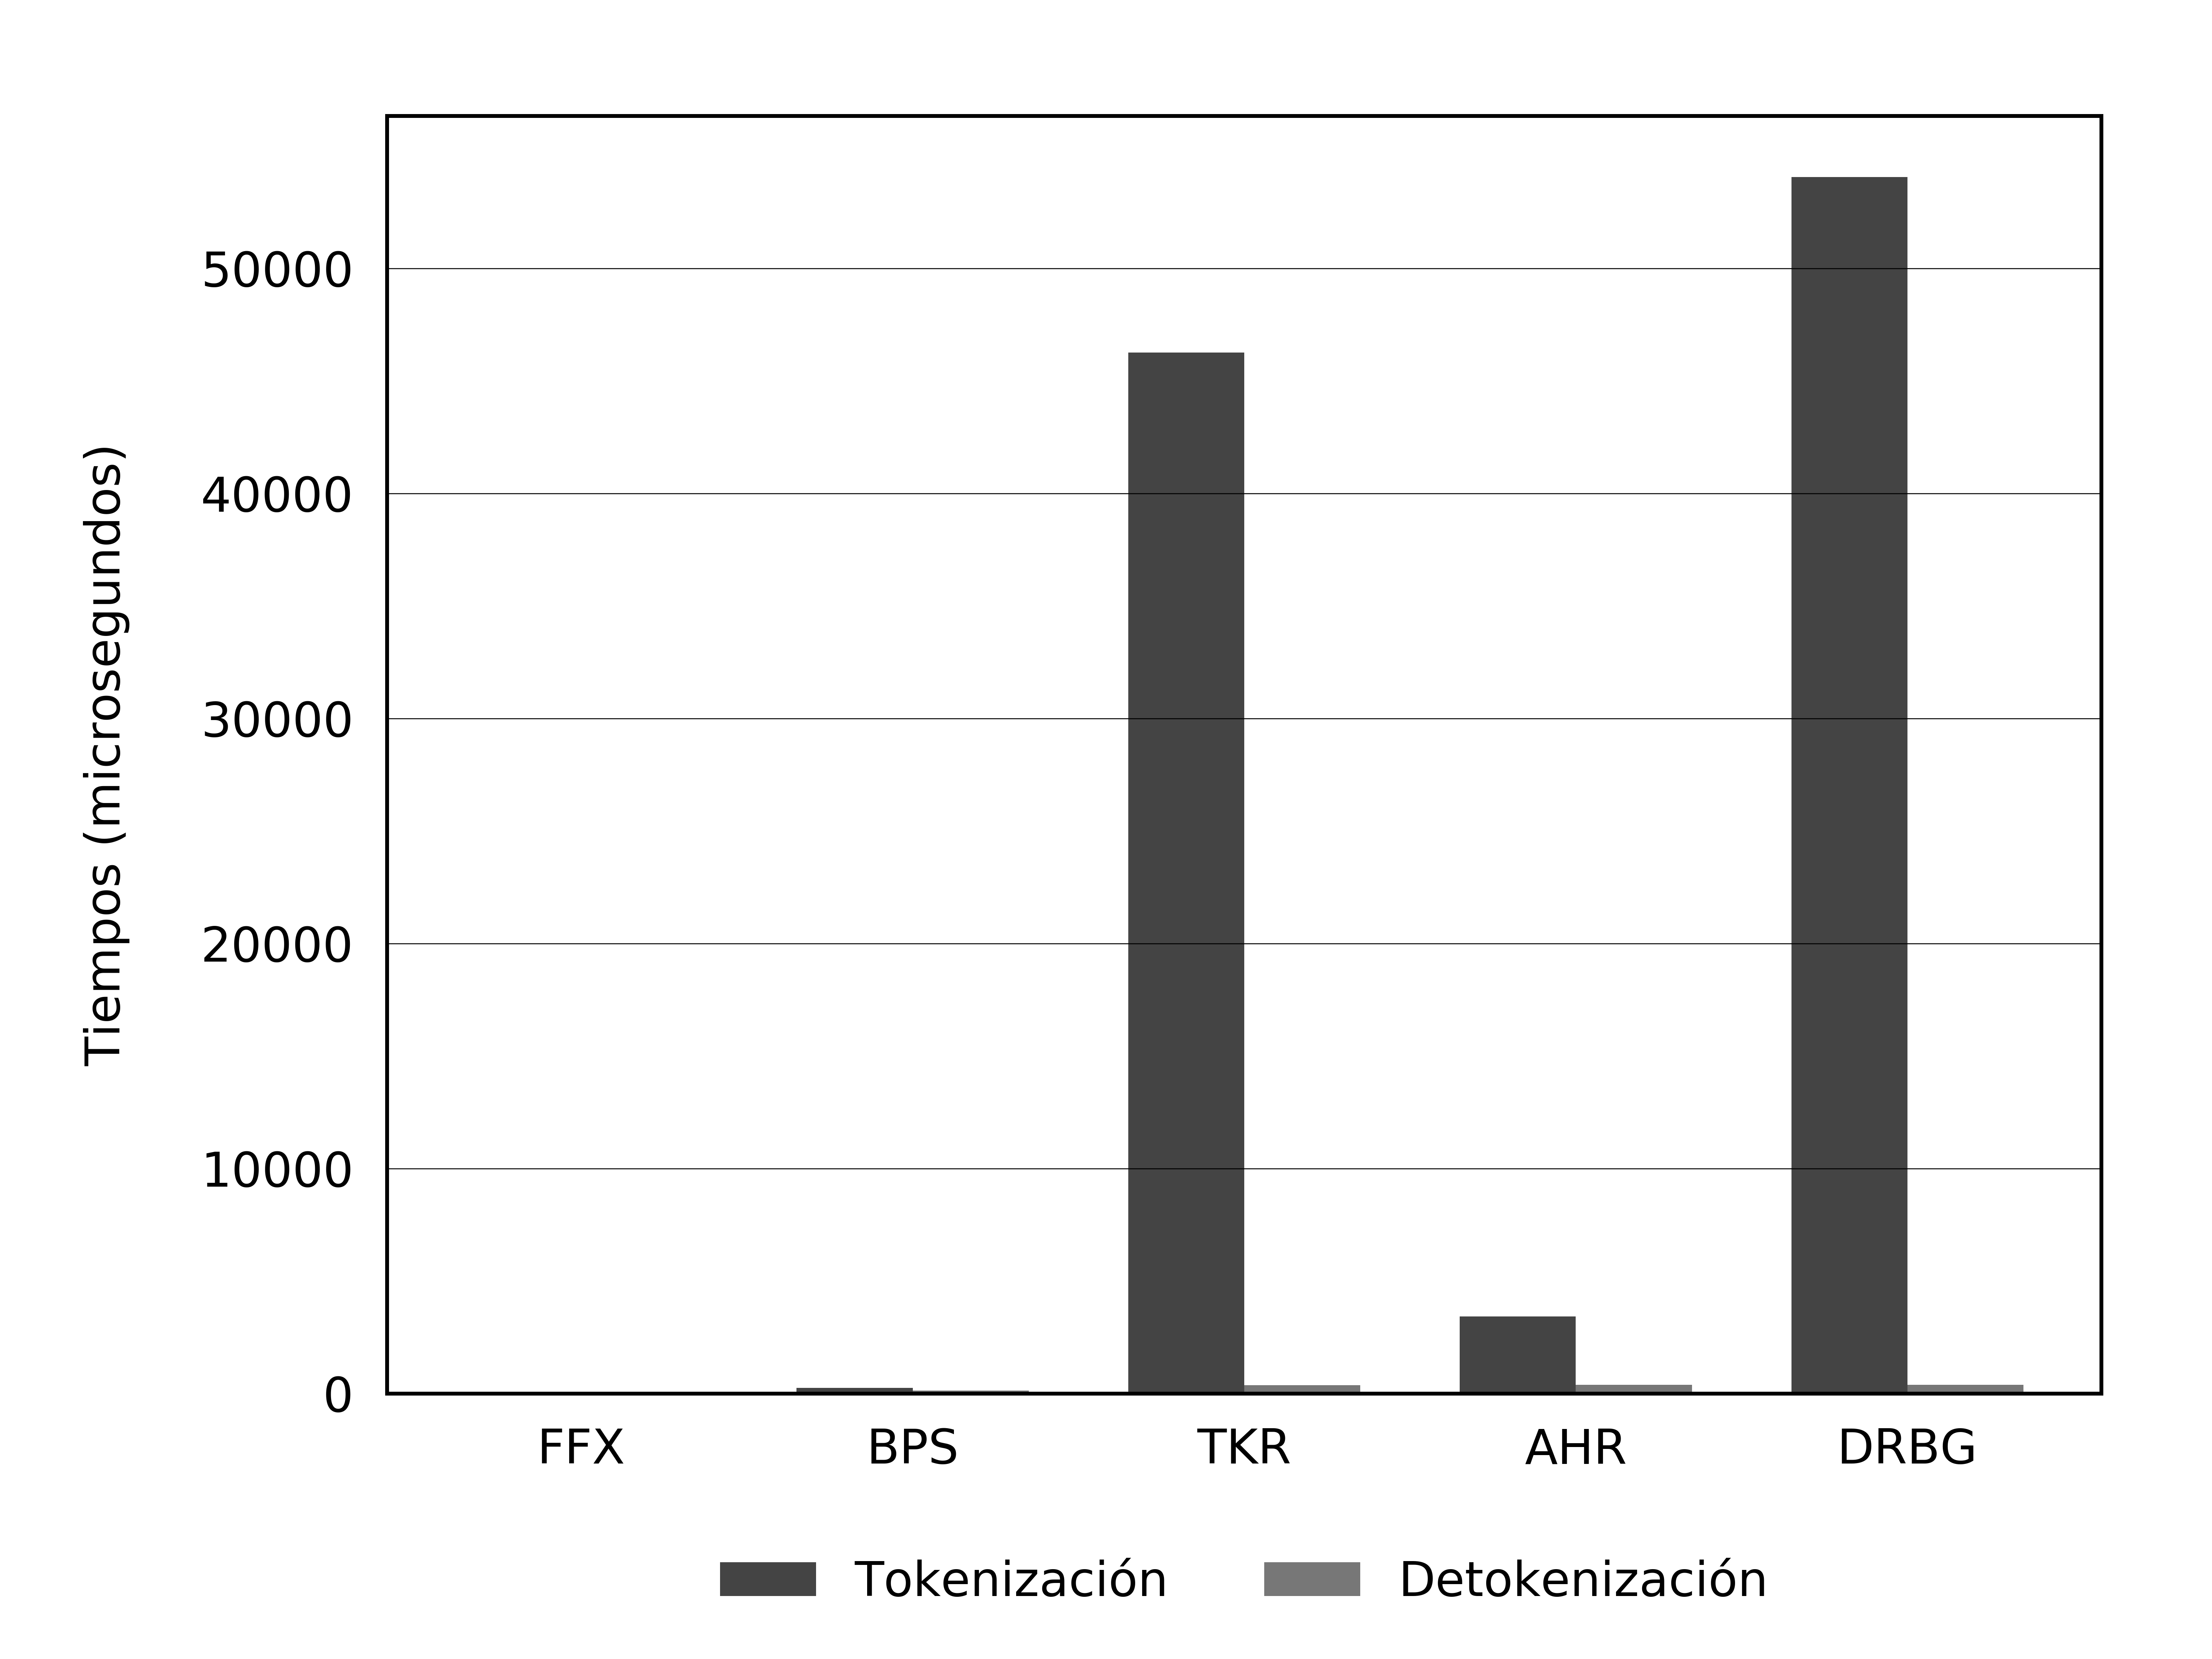
\includegraphics[width=1.0\linewidth]
      {../implementaciones/reportes/tiempos_unitarios.png}
    \caption{Comparación de tiempos de tokenización.}
    \label{figura:tiempos_tokenizacion}
  \end{center}
\end{figure}
